\section{Related Works}


Robot manipulation and grasping is an intensively researched area. The wide span of the subject makes it difficult to categorize all different approaches under one umbrella. Nevertheless, analytical and empirical grasping approaches tend to be the most used categorization in the literature \cite{Sahbani2012}.  


\subsection{Analytical Grasping Approach}

The analytical approach has been introduced first by Nguyen. He tried to solve the grasping problem by defining analytical objectives, such as a successful grasp should achieve force closure and satisfy the stability conditions by closing the object from each direction \cite{Nguyen1987}. Nguyen modeled the hand and the object, to be grasped, to compute the stable force closure grasp analytically. This kind of analytical technique comes with an exhaustive computational burden. Although the proposed algorithm works fast and correct on planar objects, they do not scale to household objects such as mugs or bottles \cite{Sahbani2012}. Moreover, in most robotics setups, full geometrical models of the objects are not available \cite{Schmidt2018}. 

\begin{figure}

    \begin{subfigure}{0.31\textwidth}
      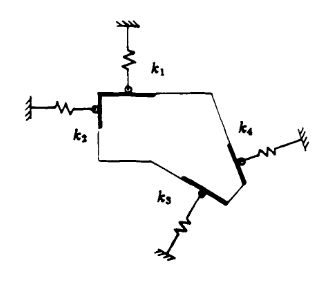
\includegraphics[width=\linewidth]{figures/graspA.png}
      \caption{} \label{fig:1a}
    \end{subfigure}%
    \hspace*{\fill}   % maximize separation between the subfigures
    \begin{subfigure}{0.31\textwidth}
      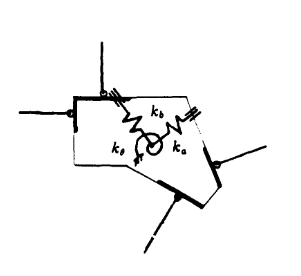
\includegraphics[width=\linewidth]{figures/graspB.png}
      \caption{} \label{fig:1b}
    \end{subfigure}%
    \hspace*{\fill}   % maximizeseparation between the subfigures
    \begin{subfigure}{0.31\textwidth}
      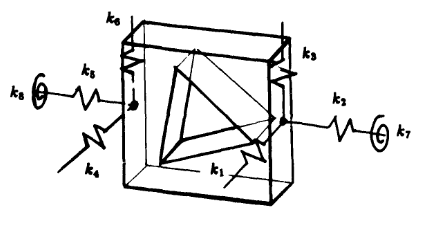
\includegraphics[width=\linewidth]{figures/graspC.png}
      \caption{} \label{fig:1c}
    \end{subfigure}

\caption{Stable force closure examples are represented as virtual springs. Nguyen proved that all force closures could be modified to be a stable grasp candidate\cite{Nguyen1987}.} \label{fig:1}
\end{figure}

\subsection{Empirical Grasping Approach}


The empirical grasping approach was introduced to overcome the difficulties faced with the analytical grasping approach. Empirical methods include learning, which is based on sampling and training. Some examples of empirical grasping approaches are imitating a human teacher \cite{Ekvall2004}, learning from the handcrafted features \cite{Saxena2008},  and deep reinforcement learning (RL) technique to learn close-loop dynamic visual grasping strategies \cite{Kalashnikov2018}. Imitating a human teacher can quickly learn the demonstrated training data. However, it has difficulties to scale to the novel objects, which were not seen during the training \cite{Sahbani2012}. Saxena et al.'s technique to learn from the feature effectively generalizes to unseen objects, but it fails to choose the best grasp for a particular task \cite{Sahbani2012}. 

RL approaches learn a thorough grasp of an object based on a definition of a goal. Thus, the learned grasp of an object is already linked to the task's goal. The flexibility of RL made itself attractive among grasping researchers. One disadvantage of the RL approach is that it requires a considerable amount of data to train. Although recent applications introduced randomization for sim-to-real transfer of the models \cite{Andrychowicz2020}, it still has difficulties to perform reliably in the real-world \cite{Caldera2018}.

\section{Learning applications on grasping}

Having experts implement handcrafted features and hand-coded controllers is time-consuming and lack generalization. Among all other approaches, machine learning applications on grasping have proven to have a high success rate on novel objects.


\subsection{Deep Learning for Detecting Grasps candidates}
Lenz et al. propose a five parameters model trained by supervised learning from the candidate grasps database. They draw a rectangle box representing the best grasp location with the five-dimensional parameter model, x, y coordinates, width, height, and orientation.

Their cascaded network architecture bypasses the need for handcrafted features. After training, the first layer network learns low-level features and delivers possible naïve grasping candidates, and the second layer chooses the top-ranked grasping candidate \ref{fig:deeplearngrasp}.

Although they achieved up to \(90\%\) success rate on grasping lab tools, this method is limited to only parallel plate gripper. It does not generalize to use other gripper types, unless the dataset is entirely updated for these grippers. Besides data collection process is time-consuming and biased.

\begin{figure}[htbp]
    \centering
    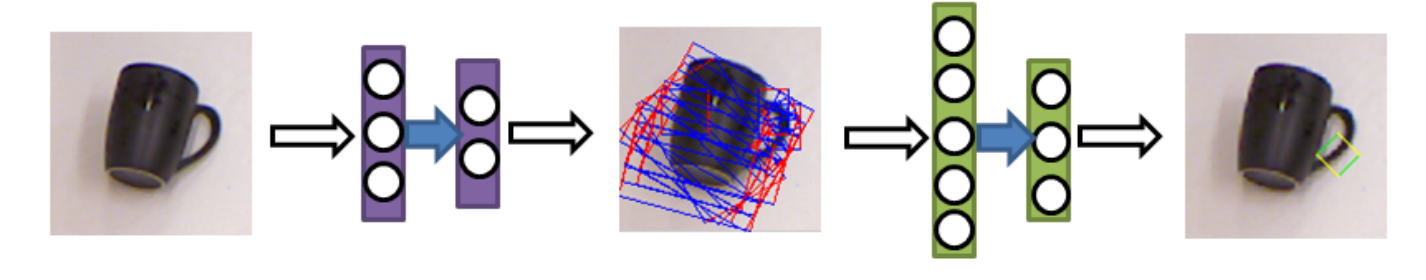
\includegraphics[width=1.\textwidth]{figures/DeepLearningGrasp}
    \caption{Red-blue rectangles represent possible grasp candidate. Green rectangle is the top-ranked grasp rectangle \cite{Lenz2013}}
    \label{fig:deeplearngrasp}
\end{figure}

\subsection{Dex-net}

Another approach for grasping is to learn the grasp robustness factor. Mahlet et al.  trained convolutional neural networks to learn the grasps robustness function from 6.7 million point cloud data. They collected the data similarly to Lenz et al. with an analytical grasp metric to evaluate the grasp's quality. 

\begin{figure}[htbp]
    \centering
    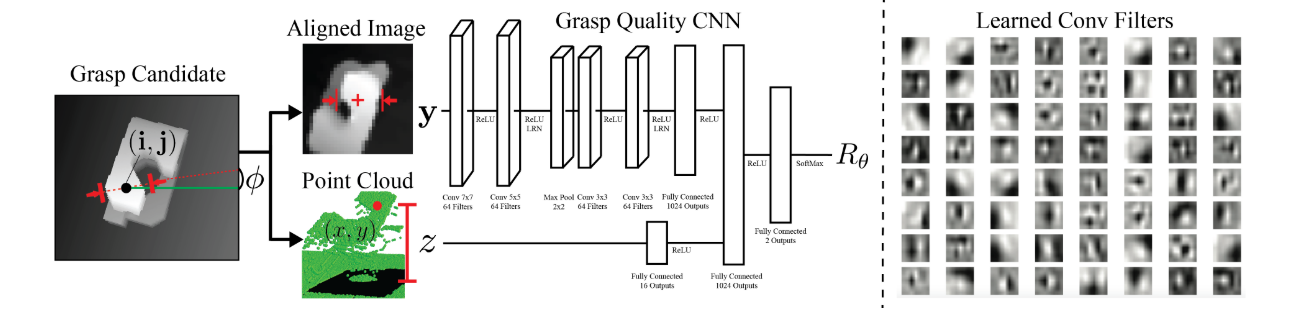
\includegraphics[width=1.\textwidth]{figures/dexnet}
    \caption{Dex-net architecture \cite{Lenz2013}}
    \label{fig:dexnet}
\end{figure}

With \(98\%\) success rate, their approach indeed proved to be robust. However, the designed network only outputs the grasp location, thus a grasp planning algorithm is needed to complete the grasping process. Moreover, data collection can be tedious due to large number of machine-labeled dataset.


\subsection{Deep Reinforcement Learning for Vision-Based Robotic Grasping: A Simulated Comparative Evaluation of Off-Policy Methods}

The sequential decision-making process is inherent in all grasping tasks. This property of grasping motivates us to model it with a reinforcement learning framework. Unlike other works, this approach trains end-to-end policies to automatically learn to grasp without any prior knowledge about the environment or the gripper model. Moreover, their system's end-to-end nature eliminates the need for additional grasp planner, which was a default in previous works. 
Quillen et al. showed that off-policy RL can increase the robustness of grasping models. Based on their investigation, corrected Monte Carlo and Deep-Q-Learning outperformed the earlier supervised learning approach. They observe that model-free RL approaches allow pre-grasp manipulation to increase the chances of grasp in future actions. 

\begin{figure}[htbp]
    \centering
    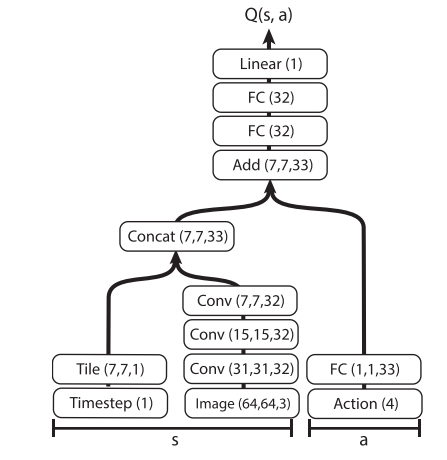
\includegraphics[width=0.5\textwidth]{figures/dql}
    \caption{Deep Learning network architecture of \cite{Quillen2018}}
    \label{fig:dql}
\end{figure}

They designed one complete network to concatenate perception input and actions from two different branches \ref{fig:dql}. Although the number of parameters increases drastically with convolutional layers from the perception branch, it makes the system more compact and easier to understand.

\subsection{Comparing Task Simplifications to Learn Closed-Loop Object Picking Using Deep Reinforcement Learning}

Breyer et al.'s learning setup is similar to the Quillen et al. with one robot gripper and randomly spawned objects in the simulation. One significant difference regarding the learning setup is that Breyer et al. generates the robot gripper only until the wrist without the rest of the arm. Thus they do not need to calculate the inverse kinematics equation.

Breyer et al. enhanced the RL-based data-driven grasp approach with curriculum learning and autoencoder for perception. Thanks to the curriculum learning setup, which increases task difficulty based on the agent's current performance, they shortened the agent's time to explore the environment. In other words, curriculum learning guides the agent throughout its learning phase. Besides, with autoencoder in the perception layer, their network tends to spend less time comprehending the observation compared to the Quillen et al. 's approach. 

Unlike Quillen et al., they experimented with an on-policy RL algorithm, TRPO. Policy-based algorithms tend to
explore better than epsilon greedy based exploration. This property may also contribute to the higher success rate and faster convergence. After training grasping models in simulation, they tested them on a real robot. Although they did not use domain randomization to minimize the reality gap, they achieved up to \(78\%\) success rate on real hardware.

\begin{figure}[htbp]
    \centering
    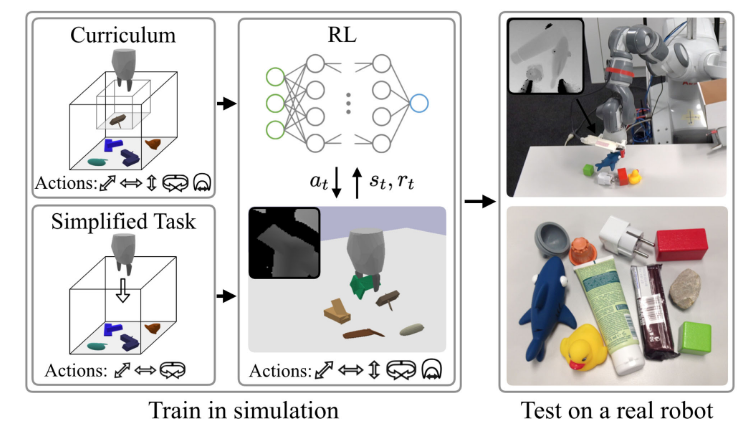
\includegraphics[width=0.7\textwidth]{figures/curriculum}
    \caption{Breyer et al. \cite{Breyer2018}}
    \label{fig:dql}
\end{figure}


\subsection{Solving Rubik's Cube With a Robot Hand}

OpenAI et al. present a novel approach for in-hand manipulation problems. Their system attacks Sim2Real discrepancy between simulated models performing on real robots. 

Training the Deep RL models on simulation is becoming more and more common. The popularity of simulation increases the demand for enhanced Sim2Real model transfer algorithms. Domain randomization has shown great success in bridging the gap between reality and simulation \cite{Tobin2017}. More researchers implement machine learning methods that randomize the environment and gripper material parameters. Through this approach, trained models can achieve higher generalization property with robustness to increasing noise at the sensor or environment settings.
OpenAI proposes a Meta-Learning method that involves memory like recurrent neural networks to learn the environment's underlying dynamics. Meta-learning and automated domain randomization algorithm combined results in an enhanced model transfer to real-world robots.

\begin{figure}[htbp]
    \centering
    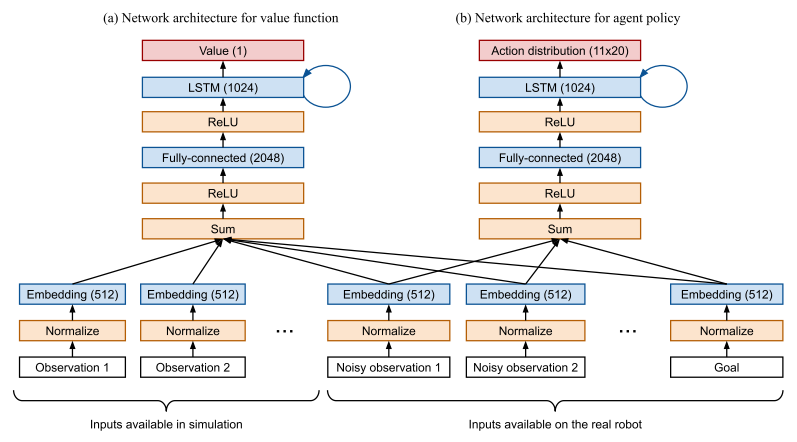
\includegraphics[width=1.\textwidth]{figures/openai}
    \caption{OpenAI policy and value network architecture \cite{openai2019rubiks}}
    \label{fig:dql}
\end{figure}